\section{Evaluation}
\label{sec:evaluation}

This section describes the evaluation process and presents the results of the evaluation. In order to run the evaluation we created a small Java project called \verb|evaluator|. It contains the classes to evaluate the performance of the recommender discussed in this report and the Top Popular recommender (see section \ref{sec:baseline}).

Evaluation is important because:
\begin{itemize}
  \item It allows us to decide if the quality of the recommender engine archives the desired results. 
  \item We are able to compare the discussed approach to other recommender algorithms. 
  \item Evaluation allows us to adjust the parameters in order to get better results.
\end{itemize}

\subsection{How to measure the performance of the \gls{topnt}?}

Most commonly accepted evaluation measure for recommender systems is the Mean Average Error or Root \gls{mae} of the predicted ratings and the actual one \cite{Ricci}\cite{jannach11}.
As described in section \ref{sec:problem} the \gls{rec} does not estimate preference values. It produces a \glspl{topn}. Hence we can not use \gls{mae} as a performance metric. 

\begin{figure}
\centering
\begin{tikzpicture}[
box/.style={draw,rectangle,minimum size=3cm,text width=2.5cm,align=left}]
\matrix (conmat) [row sep=.1cm,column sep=.1cm] {
\node (tpos) [box,
    label=left:Relevant items,
    label=above:,
    ] {relevant \\and\\recommended \\ (TP)};
&
\node (fneg) [box,
    label=above:,
    label=above right:,
    label=right:] {relevant\\ but not \\recommended\\(FN)};
\\
\node (fpos) [box,
    label=left:irrelevant items,
    label=below left:,
    label=below:Top-N list] {irrelevant \\but\\recommended};
&
\node (tneg) [box,
    label=right:,
    label=below:not in Top-N list] {irrelevant\\and not\\recommended};
\\
};
\node [left=.05cm of conmat,text width=1.5cm,align=right] {\textbf{actual \\ prefences}};
\node [above=.05cm of conmat] {\textbf{recommender classification}};
\end{tikzpicture}
\caption{Confusion matrix for top-N recommendation task}
\label{fig:confusionmatrix}
\end{figure}

We can look at the recommender problem as a classification problem. The recommender engine assigns every item into the category of recommendable items or unimportant items.
If we look at the recommender problem as a classification problem we can make use of precision and recall to evaluate the performance. Precision and \gls{recall} are two \gls{ir} concepts \cite{Manning}. We provide a brief summary here to each of these measures.

Precision and recall depend on the following measures.
\begin{description}
\item[True positive (TP)] Number of items classified as recommendable or relevant that are truly of interest to the user. 
\item[True negatives (TN)] Number of instances not contained in the \gls{topn} (classified as irrelevant) and that in fact are not of interest to the user.
\item[False positives (FP)] Number of instances recommended but are not relevant to the user.
\item[False negatives (FN)] Number of instances not shown in the \gls{topn} but that in fact are relevant to the user.
\end{description}


Figure \ref{fig:confusionmatrix} visualizes the measures used for precision and recall. This table is called confusion matrix or contingency table \cite{Manning}. 

\subsubsection{Precision and Recall}
\label{sec:precision}

\begin{description}
\item[Precision] Precision is the proportion of items in the \gls{topn} that are relevant \cite{Manning}.
  \begin{equation}
    \label{eq:precision}
    \text{Precision} = \frac{\text{number relevant items recommended}}{\text{size of the recommendation list}}
  \end{equation}
We can formulate this with the measures from the confusion matrix.
  \begin{equation}
    \label{eq:precisionm}
    \text{Precision} = TP/(TP+FP)
  \end{equation}

 Suppose the recommender create a list of 5 items. If 3 items are relevant recommendations then the precision is $3/5$. 
Precision only considers the accuracy of the recommendation list and not the comprehensiveness of the result.

\item[Recall] Recall is the proportion of relevant items that appear in the \gls{topn}. 
  \begin{equation}
    \label{eq:recall}
    \text{Recall} = \frac{\text{number relevant items recommended}}{\text{relevant items}}
  \end{equation}
  \begin{equation}
    \label{eq:recallcm}
    \text{Recall} = TP/(TP+FN)
  \end{equation}
Suppose there are 9 relevant recommendations. If the recommender results contains 3 of these relevant recommendations then the recall is 3/9.

Note that recall should not used without precision. We could build a recommender with perfect recall by recommending all items.
\end{description}

\subsubsection{Implementation}
\label{sec:irimpl}

Listing \ref{lst:irstats} shows the implementation of precision and recall. 
The variable \verb|rec| contains an object of type \verb|Recommender|. \verb|Recommender| provides the method \verb|recommend|. \verb|recommend| takes the ID of the active user and the size $N$ of the top-N list as parameters. The argument \verb|topNsize| corresponds to $TP+FP$. It returns a top-N list for the active user. 

The variable \verb|relevantItem| contains a list with relevant items for the active user.

We count how many items in the top-N list are also in the list \verb|relevantItems| and assign the result to \verb|relevantItemsRetrieved|. \verb|relevantItemsRetrieved| corresponds to the $TP$ value. In order or compute precision or recall we divide \verb|relevantItemsRetrieved| by \verb|topNsize| or the size of the collection\\ \verb|relevantItems|.


\begin{lstlisting}[caption=Implementation of precision and recall,label=lst:irstats]
double precision = 0;
double recall = 0;
int relevantItemsRetrieved = 0;

List<RecommendedItem> recItems = rec.recommend(userID, topNsize);
   for (RecommendedItem recItem : recItems) {
	if (relevantItem.contains(recItem.getItemID())){
			relevantItemsRetrieved++;
	}
   }

// Precision
int numRecommendedItems = reItems.size();
precision = ((double) relevantItemsRetrieved / (double) topNsize);
		      
// Recall
recall =  relevantItemsRetrieved / (double) relevantItems.size());
		      
\end{lstlisting}

\subsection{Testing Methodology}
\label{sec:methodology}
The definitions \ref{eq:precision} and \ref{eq:recall} of precision in recall rely on the number of relevant items.
If we want to evaluate a recommender with \gls{precision} and \gls{recall}, we have to define, what is a relevant item for the active user. 

Relevancy depends on the goal of the recommender. For example, an item is relevant if the user would give it a high rating or if he would purchase the item but he is not aware of it.
Those items are unknown at the time of the recommendation. 

Unfortunately we do not know if a user likes some new item in the future.
But we can simulate the preferences of the future by setting aside a small part of the real data set as test data.

In order to separate the test data set from the training data set we get all ratings of user $u$. We sort these rating according the rating value. Then we select the top $N$ items $T$ that are greater then a given threshold $t$ from the sorted list. Items in $T$ have a high rating and we assume they are relevant to the user $u$. Items in $T$ form the set $TP + FN$ (see figure \ref{fig:confusionmatrix}). 
The threshold prevents us from adding items with a low rating to $T$. If a user rates three items with the rating 5.0, 1.0 and 1.0 the evaluation algorithm would add the items with the bad rating 1.0 to $T$. Hence the items with bad rating 1.0 lead to lower recall measures. 
If there are no numerical rating values but only Boolean values we have to select $N$ items at random.

All ratings in $T$ are removed from the overall input set. The remaining preferences form the training data set $M$. In order to measure precision and recall we first train the recommender with the data in $M$. For instance, if we evaluate the co-occurrence based recommender we compute indicator matrix from section \ref{sec:llr} with $M$.

We use the trained recommender to form the \gls{topn} for user $u$. This list corresponds to the set $TP + FP$ in the confusion matrix.

We check how many items are contained in the top-N list that are in $T$ with the implementation from section \ref{sec:irimpl}. These items are the set $TP$ (see figure \ref{fig:confusionmatrix}). 

For example, if $N$ is 5 this would mean \gls{precision} and recall are evaluated by removing the top 5 preferences for a user and then finding the percentage of those 5 items included in the top-N recommendation list for that user. 

In short the evaluation process for a single user $u$ can be divided into several steps:
\begin{enumerate}
\item Retrieve relevant items $T$ for user $u$ ($TP+FN$).
\item Build the training set $M$ by removing the corresponding preferences from input data set.
\item Train the recommender engine with $M$.
\item Form a \gls{topn} for $u$ ($TP+FP$).
\item Count the number of items that appear in the top-N list and in $T$ ($TP$).
\item Compute precision and recall based on $TP$, $FP$ and $FN$.
\end{enumerate}

The evaluation process has the following parameters:
\begin{description}
\item[Size of the result] The length $N$ of recommendations list and number of the relevant items. 
\item[Relevance threshold] Determines if an item is relevant or not.
\end{description}

\subsection{Baseline algorithms}
\label{sec:baseline}

In order to get a feel what values of precision and recall to expect and to determine the performance of the \gls{rec} we compare it with three base line algorithms. 

\begin{description}
\item[Random] The recommender randomly recommends $N$ items to the user. This algorithms serves just as baseline for the more complex algorithms.
\item[TopPopular]  It creates a list of items ordered by the numbers of ratings for a specific item. TopPopular is a non-personalized recommender because it presents the same list of items to any user \cite{Cremonesi}. Listing \ref{lst:toppop} shows the implementation of the the TopPopular algorithm. 

\begin{lstlisting}[label=lst:toppop, caption={Implementation of top popular recommender}]
Map<Long, Integer> item2pop = new HashMap<Long, Integer>();
LongPrimitiveIterator iter = dataModel.getUserIDs();
while (iter.hasNext()) {
PreferenceArray prefs = dataModel.getPreferencesFromUser(iter
	.nextLong());
for (int i = 0; i < prefs.length(); i++) {
	Integer counter = item2pop.get(prefs.getItemID(i));
	if (counter == null) {
		item2pop.put(prefs.getItemID(i), 1);
	} else {
		item2pop.put(prefs.getItemID(i), counter + 1);
	}
      }
}
List<RecommendedItem> popitems = transfom2list(item2pop);
Collections.sort(itemidcounter, new RecommenderItemComparator()); 
return popitems
\end{lstlisting}

\item[Item-based with cosine similarity]  \Gls{itembased} collaborative filtering is a model-based, collaborative filtering algorithm. It computes the similarities between all items and predicts user preferences based on existing ratings. We use the cosine similarity \cite{ekstrand11} to measure the similarity between two items. The \gls{itembased} algorithm selects $k$ nearest neighbors $N$ of an item $i$ that the user $u$ already rated. It then weights the ratings of the active user $u$ for each item $i'$ in $N$ with the similarity $sim(i,i')$ and compute the sum of that. The predicted rating $r_{u,i}$ for user $u$ and item $i$ is the normalized value of the sum \cite{jannach11}:

\end{description}
\begin{equation}
  \label{eq:computeprediction}
  r_{u,i} = \frac{\sum_{i' \in N}{sim(i,i') r_{u,i}}}{\sum_{i' \in N}{|s(i,i')|}}
\end{equation}

We use Mahout's implementation of an \gls{itembased} recommender. Mahout provides the \verb|GenericItemBasedRecommender| class with an implementation of an \gls{itembased} recommender. To compute the similarity we use \verb|UncenteredCosineSimilarity|.

\subsection{Dataset}
\label{sec:dataset}

The testing methodology of section \ref{sec:methodology} requires an existing data set. We used ratings and tagging activity from MovieLens, a movie recommendation service \cite{movielensdata}.
MovieLens data sets were collected by the GroupLens Research Project at the University of Minnesota. The data was collected through the MovieLens web site (movielens.umn.edu) during the seven-month period from September 19th, 1997 through April 22nd, 1998 \cite{movielensdata}.

This data set consists of:
\begin{itemize}
\item 100,000 ratings. The ratings are scores from 1 to 5. A rating is made by one user to one movie at a specific time. 

\item 943 users. Each user has rated at least 20 movies
\item 1682 movies. Movies are categorized in genres. A movie has an ID, a title, and a list of associated genres. 
\item 2488 \gls{tag} applications. A \gls{tag} is applied by one user to one movie at a specific time. Tags are user-generated meta data about movies. Each tag is typically a single word or short phrase. 
\end{itemize}
 
We choose this data set due to several reasons:
\begin{itemize}
\item It contains ratings and tagging activity. Hence we can use two indicators for the multimodal co-occurrence based recommender.
\item As described in section \ref{sec:methodology} we need numerical rating scores to select the top $N$ ratings of a user in order to form a test set. 
\item  It is common to evaluate a recommender engine with it. Hence it is easier to compare the results with other recommender engines. 
\end{itemize}


\subsubsection{Simulating user action "like"}

The \gls{rec} takes user actions as Boolean values as an input. The MovieLens data set contains preferences with a numerical rating score. 
In order to simulate the user action ``like'' as described in section \ref{sec:inputdata} we generate a new data set based on the MovieLens data set. We select all preferences with a score equal or above 4.0. These \glspl{preference} indicate that the user likes the item hence we consider them as likes.

\subsection{Evaluationresults}
\label{sec:results}
To compare the performance of the \glspl{rec} with variable number of \glspl{indicator} and therefore measure the impact of an additional indicator we evaluated three different recommenders. 

\begin{description}
\item[\Gls{coocc} user likes] It only considers \gls{coocc} of the user's action \gls{like} as described by equation \ref{eq:recommendation} (section \ref{sec:problem}).
\item[\Gls{coocc} of likes and tags] In addition to likes we use tag-associations to compute the similarity as described by equation \ref{eq:multi}. We use the tags associated with an item to compute a tag \gls{indicator} matrix and store these indicator in a separate field in Solr. We add tags that are associated with the \gls{au} to the query.
\item[\Gls{coocc} of likes, tags and user ratings] We use the \gls{coocc} based similarity metric described in section \ref{sec:llr} to compute similarity based on all preferences from the MovieLens data set. We can count \gls{coocc} of preferences between items and ignore the score value. To query this \gls{indicator} field we use the user's recent likes.
\end{description}

We measure precision and recall at $N=10$ for all three recommenders and the baseline algorithms. Hence we retrieve a list of 10 items. Relevant items are the 10 best rated items above the threshold. For every user we compute his average rating value $\mu$ and the standard deviation $\sigma$. We set the threshold to $\mu + \sigma$.

\pgfplotsset{width=7cm}
\begin{figure}
  \centering
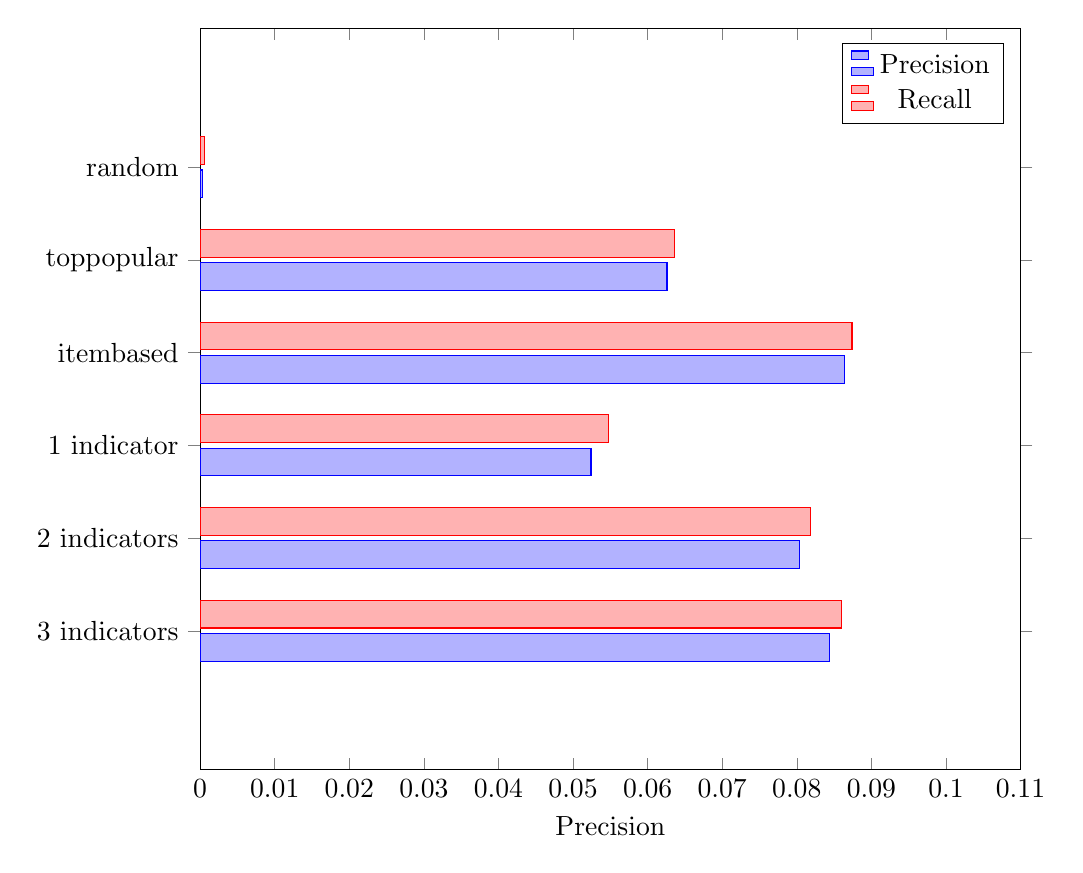
\begin{tikzpicture}
\begin{axis}[
xbar,
xmin=0,
xmax=0.11,
width=12cm,
height=11cm,
enlarge y limits=0.3,
xlabel={Precision},
symbolic y coords={3 indicators,2 indicators,1 indicator,itembased,toppopular,random},
ytick=data,
x tick label style={/pgf/number format/fixed}
]

\addplot coordinates {(0.00035,random) (0.0626,toppopular) (0.0864,itembased) (0.0524,1 indicator) (0.0804,2 indicators) (0.0844,3 indicators)};
\addplot coordinates {(0.00054,random) (0.0636,toppopular) (0.0874,itembased) (0.0547,1 indicator) (0.0818,2 indicators) (0.086,3 indicators)};
\legend{Precision, Recall};
\end{axis}
\end{tikzpicture} 
\caption{Precision and recall comparison of the recommender algorithms, random generated recommendations, Top Popular, itembased  and three \glspl{rec} with a variable number of indicators with precision at 10 and $N$ = 10 (number of recommended items)}
  \label{fig:precisionrecallvalues}
\end{figure}

Figure \ref{fig:precisionrecallvalues} shows the comparison of \glspl{rec} with one, two and three indicators with the baseline algorithms from section \ref{sec:baseline}.
The multimodal \gls{rec} with all indicators achieves an average precision and recall of 8.6 and 8.4 percent. This seems low. The recommender rarely recommends an item that the user liked explicitly. On the other hand we do not know if the recommended items are appealing to the user if he never rated them.

The evaluation shows that the quality of the recommender increases when we take more indicators into account. If we use just the user action ``like'' precision and recall are 5.2 and 4.5 percent. If we use the user action like and \glspl{tag} as indicator precision and recall are  8.1 and 8 percent. That is an increase of 55 and 85 percent.

Compared to the baseline algorithms the \gls{coocc} based recommender with three indicator achieves the best results. It performs slightly better than the \gls{itembased} algorithm. The reason for this is that the \gls{rec} has access to more information than the \gls{itembased} algorithm that only uses preferences and no tags.

Another interesting fact is that the non-personalized algorithm almost match the quality of the more sophisticated approaches. Compared to randomly generated recommendations the \gls{coocc} improves the quality with a factor of about 250.
